\chapter{Results}
\label{c:result}

\section{Datasets}

%
% GSE52194 Breast cancer

GSE52194 \cite{eswaran2012:transcriptomic}
Table~\ref{tab:dataset-breast}

\begin{table}[!htbp]
    \caption[Experiment design of breast cancer GSE52194]{
        Experiment design of breast cancer dataset GSE52194.
    }
    \label{tab:dataset-breast}
    \centering
    \begin{threeparttable}
        \begin{tabular}{llr}
            \toprule
            Condition & Sample name & SRA ID and filename \\
            \midrule
            NBS      & NBS1      & SRR1027188 \\
            NBS      & NBS2      & SRR1027189 \\
            NBS      & NBS3      & SRR1027190 \\
            TNBC     & TNBC1     & SRR1027171 \\
            TNBC     & TNBC2     & SRR1027172 \\
            TNBC     & TNBC3     & SRR1027173 \\
            TNBC     & TNBC4     & SRR1027174 \\
            TNBC     & TNBC5     & SRR1027175 \\
            TNBC     & TNBC6     & SRR1027176 \\
            Non-TNBC & Non-TNBC1 & SRR1027177 \\
            Non-TNBC & Non-TNBC2 & SRR1027178 \\
            Non-TNBC & Non-TNBC3 & SRR1027179 \\
            Non-TNBC & Non-TNBC4 & SRR1027180 \\
            Non-TNBC & Non-TNBC5 & SRR1027181 \\
            Non-TNBC & Non-TNBC6 & SRR1027182 \\
            HER2     & HER2-1    & SRR1027183 \\
            HER2     & HER2-2    & SRR1027184 \\
            HER2     & HER2-3    & SRR1027185 \\
            HER2     & HER2-4    & SRR1027186 \\
            HER2     & HER2-5    & SRR1027187 \\
            \bottomrule
        \end{tabular}
    \end{threeparttable}
\end{table}



% GSE52778 Airway Muscle and Asthma

GSE52778 \cite{himes2014:rnaseq}
Table~\ref{tab:dataset-airway}

\begin{table}[!htbp]
    \caption[Experiment design of GSE52778 airway muscle dataset]{
        Experiment design of GSE52778 airway muscle dataset.
    }
    \label{tab:dataset-airway}
    \centering
    \begin{threeparttable}
        \begin{tabular}{llr}
            \toprule
            Condition & Sample name & SRA Accession ID \\
            \midrule
            Untreated & N61311\_Untreated  & SRR1039508 \\
            Untreated & N052611\_Untreated & SRR1039512 \\
            Untreated & N080611\_Untreated & SRR1039516 \\
            Untreated & N061011\_Untreated & SRR1039520 \\

            Dex       & N61311\_Dex        & SRR1039509 \\
            Dex       & N052611\_Dex       & SRR1039513 \\
            Dex       & N080611\_Dex       & SRR1039517 \\
            Dex       & N061011\_Dex       & SRR1039521 \\

            Alb       & N61311\_Alb        & SRR1039510 \\
            Alb       & N052611\_Alb       & SRR1039514 \\
            Alb       & N080611\_Alb       & SRR1039518 \\
            Alb       & N061011\_Alb       & SRR1039522 \\

            Alb\_Dex  & N61311\_Alb\_Dex   & SRR1039511 \\
            Alb\_Dex  & N052611\_Alb\_Dex\tnote{$\dagger$} & SRR1039515\tnote{$\dagger$} \\
            Alb\_Dex  & N080611\_Alb\_Dex  & SRR1039519 \\
            Alb\_Dex  & N061011\_Alb\_Dex  & SRR1039523 \\
            \bottomrule
        \end{tabular}
        \begin{tablenotes}
        \item[$\dagger$] This sample was excluded from the later-on analyses
            since its pair-end sequencing reads were mismatched.
        \end{tablenotes}
    \end{threeparttable}
\end{table}



\section{Account registration}

TODO: Screenshot groups here.

\section{Data source discovery}

% checksum check

\section{Experiment design}

% condition
% simple and advanced mode

\section{Analysis submission}


\section{Job queue monitoring}

% email notification

\section{Report and result access}

\subsection{Integration with public genome browser}


\section{RNA-Seq analysis result}

\subsection{QC}

\subsection{Alignment - STAR}

\subsection{Alignment - HISAT2}

TODO: finish the dataset execution

\subsection{Cufflinks}

\subsection{featureCounts}

\subsection{DESeq2}

TODO: finish the dataset execution


\section{DNA-Seq analysis result}

\subsection{QC}

\subsection{Alignment - BWA MEM}

\subsection{Variant calling - Varscan}

\subsection{Variant calling - GATK}

TODO: finish the data execution

% There is a tree in Figure~%\ref{i:tree}.
% This is English line spacing test. You should see double spacing text.
% This is English line spacing test. You should see double spacing text.
% This is English line spacing test. You should see double spacing text.

%i:tree
%\begin{figure}[!htbp]
\centering
\tikzset{every tree node/.style={align=center},
    level distance=40pt,
    sibling distance=6pt}
\begin{tikzpicture}
\Tree[.root
       [ (a) ]
       [.node
         [.node
           [ (b) ]
           [ (c) ]
         ]
         [.node
           [ (d) ]
           [ (e) ]
           [ (f) ]
           [ (g) ]
           [ (h) ]
         ]
       ]
     ]

\end{tikzpicture}

\caption{A tree. }
\label{i:tree}
\end{figure}


% There is a barchart in Figure~%\ref{i:barchart}.
% This is English line spacing test. You should see double spacing text.
% This is English line spacing test. You should see double spacing text.
% This is English line spacing test. You should see double spacing text.

%i:barchart
%\begin{figure}[!htbp]
    \centering
    \vspace{2em}
    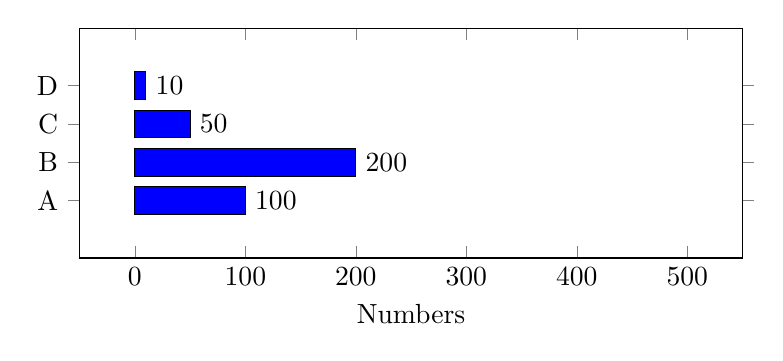
\begin{tikzpicture}
        \begin{axis}[
            enlarge y limits=0.5,
            enlarge x limits=0.1,
            height=4.5cm,
            width=10cm,
            symbolic y coords={A,B,C,D},
            xmin=0,
            xmax=500,
            xbar=1pt,
            xlabel=Numbers,
            nodes near coords={\pgfmathprintnumber[/pgf/number format/assume math mode]{\pgfplotspointmeta}},
            nodes near coords align={horizontal},
            every node near coord/.append style={
                anchor=west}
            ,
            xticklabel style={/pgf/number format/assume math mode},
            yticklabel style={/pgf/number format/assume math mode},
            ytick=data
          ]
            \addplot[xbar,fill=blue] coordinates {
            (100,A)
            (200,B)
            (50,C)
            (10,D)
            };
        \end{axis}
    \end{tikzpicture}
    \caption{A barchart.}
    \label{i:barchart}
\end{figure}


% Our method outperforms state-of-art systems as shown in Table~\ref{t:results}.
% This is English line spacing test. You should see double spacing text.
% This is English line spacing test. You should see double spacing text.
% This is English line spacing test. You should see double spacing text.

%t:results
% \begin{table}[!htbp]
\caption{Final performance of our system. }
\label{t:results} 
\centering
\begin{tabular}{|c|c|c|c|}
\hline

Method      &    Precision &     Recall &     F1-Score \\ \hline
their model &     3.40     &      3.40  &      3.40    \\ \hline
our model   &    99.99     &     99.99  &     99.99    \\ \hline


\end{tabular}
\end{table}

% \begin{table}[!htbp]
\caption[mirDeep2 result summary of both novel and known miRNA.]{mirDeep2 result summary of both novel and known miRNA. Here we can put some very lengthy descriptions as our table legend, and it will not ruin the list of tables, which will only display the shorten version of the caption.}
\label{t:all-sum}
\centering
\begin{threeparttable}
	\begin{tabular}{ccccccc}
	\toprule
    & \multicolumn{3}{c}{novel miRNAs} & \multicolumn{3}{c}{known miRNAs}\\
    \cmidrule(r){2-4} \cmidrule(r){5-7}
    miRDeep2 &       & estimated & estimated  &       &       &  \\
    score & predicted &  false positives\tnote{$\ast$} & true positives\tnote{$\dagger$} & in species & in data & detected\\
    \midrule
   >10    & 25    & 7 $\pm$ 3 & 18 $\pm$ 3 & 2025  & 1199  & 600 (50\%) \\
    9     & 28    & 8 $\pm$ 3 & 20 $\pm$ 3 & 2025  & 1199  & 609 (51\%) \\
    8     & 30    & 8 $\pm$ 3 & 22 $\pm$ 3 & 2025  & 1199  & 621 (52\%) \\
    7     & 31    & 8 $\pm$ 3 & 23 $\pm$ 3 & 2025  & 1199  & 635 (53\%) \\
    6     & 37    & 9 $\pm$ 3 & 28 $\pm$ 3 & 2025  & 1199  & 647 (54\%) \\
    5     & 50    & 11 $\pm$ 3 & 39 $\pm$ 3  & 2025  & 1199  & 720 (60\%) \\
    4     & 58    & 27 $\pm$ 6 & 31 $\pm$ 6 & 2025  & 1199  & 744 (62\%) \\
    3     & 64    & 74 $\pm$ 8 & 0 $\pm$ 1 & 2025  & 1199  & 752 (63\%) \\
    2     & 92    & 97 $\pm$ 9 & 2 $\pm$ 3 & 2025  & 1199  & 797 (66\%) \\
    1     & 181   & 132 $\pm$ 10 & 49 $\pm$ 10 & 2025  & 1199  & 891 (74\%) \\
    0     & 245   & 397 $\pm$ 20 & 0 $\pm$ 0 & 2025  & 1199  & 923 (77\%) \\
    -1    & 284   & 574 $\pm$ 22 & 0 $\pm$ 0 & 2025  & 1199  & 945 (79\%) \\
    -2    & 406   & 703 $\pm$ 23 & 0 $\pm$ 0 & 2025  & 1199  & 970 (81\%) \\
    -3    & 537   & 822 $\pm$ 25 & 0 $\pm$ 0 & 2025  & 1199  & 987 (82\%) \\
    -4    & 625   & 959 $\pm$ 28 & 0 $\pm$ 0 & 2025  & 1199  & 988 (82\%) \\
    -5    & 703   & 1088 $\pm$ 27 & 0 $\pm$ 0 & 2025  & 1199  & 991 (83\%) \\
    -6    & 774   & 1173 $\pm$ 26 & 0 $\pm$ 0 & 2025  & 1199  & 991 (83\%) \\
    -7    & 862   & 1227 $\pm$ 26 & 0 $\pm$ 0 & 2025  & 1199  & 992 (83\%) \\
    -8    & 923   & 1265 $\pm$ 27 & 0 $\pm$ 0 & 2025  & 1199  & 992 (83\%) \\
    -9    & 962   & 1291 $\pm$ 26 & 0 $\pm$ 0 & 2025  & 1199  & 992 (83\%) \\
    -10   & 1006  & 1311 $\pm$ 26 & 0 $\pm$ 0 & 2025  & 1199  & 992 (83\%) \\
		\bottomrule
	\end{tabular}
	\begin{tablenotes}
		\item[$\ast$] The number of false positives is estimated from 100 rounds of permuted controls.
		\item[$\dagger$] The number of true positives is estimated as $t = \mathit{total} - \mathit{false\:positives}$. The percentage of the predicted novel miRNAs that is estimated to be true positives is calculated as $p = t / \mathit{total}$. In each of the 100 rounds, $t$ and $p$ are calculated, generating mean and standard deviation of $t$ and $p$. The variable $p$ can be used as an estimation of miRDeep2 positive predictive value at the score cut-off. 
    \end{tablenotes}
\end{threeparttable}
\end{table}
% vim: set textwidth=79:
